\documentclass[11pt,a4paper]{article}
\usepackage[utf8]{inputenc}
\usepackage[english]{babel}
\usepackage{geometry}
\geometry{margin=1in}
\usepackage{graphicx}
\usepackage{hyperref}
\usepackage{minted}
\usepackage{titlesec}
\usepackage{fancyhdr}
\usepackage{caption}
\usepackage{enumitem}
\usepackage{listings}
\usepackage{xcolor}
\usepackage{float}

% Code highlighting
\lstset{
  basicstyle=\ttfamily\small,
  breaklines=true,
  backgroundcolor=\color{gray!10},
  frame=single,
}
\lstdefinelanguage{yaml}{
  keywords={true,false,null,y,n},
  keywordstyle=\color{blue},
  basicstyle=\ttfamily\small,
  sensitive=false,
  comment=[l]{\#},
  morecomment=[l]{\#},
  commentstyle=\color{gray}\ttfamily,
  morestring=[b]',
  morestring=[b]"
}
\lstdefinelanguage{dart}{
  morekeywords={
    async, await, break, case, catch, class, const, continue, default, do, else, enum, export,
    extends, external, factory, false, final, finally, for, if, implements, import, in, interface,
    is, new, null, on, override, part, rethrow, return, set, static, super, switch, this, throw,
    true, try, typedef, var, void, while, with, yield
  },
  sensitive=true,
  morecomment=[l]{//},
  morecomment=[s]{/*}{*/},
  morestring=[b]",
  morestring=[b]',
  keywordstyle=\color{blue}\bfseries,
  commentstyle=\color{gray}\ttfamily,
  stringstyle=\color{orange},
  basicstyle=\ttfamily\small,
}

% Header and footer
\pagestyle{fancy}
\fancyhf{}
\rhead{Project Documentation}
\lhead{Rocket App}
\rfoot{\thepage}

% Section formatting
\titleformat{\section}{\normalfont\Large\bfseries}{\thesection}{1em}{}
\titleformat{\subsection}{\normalfont\large\bfseries}{\thesubsection}{1em}{}

% Custom commands
\newcommand{\email}[1]{\texttt{#1}}
\newcommand{\id}[1]{\texttt{#1}}

% Title page
\begin{document}

\begin{titlepage}
    \begin{flushright}
        
\includegraphics[width=4cm]{images/Logo-HFT-Stuttgart.png}
    \end{flushright}
    \vspace*{0.5cm}

    \begin{center}
        {\Huge \textbf{Rocket App} \par}
        \vspace{0.3cm}
        {\LARGE \textit{Pervasive Computing} \par}
        \vspace{1.5cm}
        
\includegraphics[width=5cm]{images/AppIcon.png}
        \vspace{1.5cm}

        {\Large Autoren: \par}
        \vspace{0.3cm}
        \begin{tabular}{rl}
            Paul Durz      & \email{22dupa1bif@hft-stuttgart.de} \\
                          & Matrikelnummer: \id{1005080} \\
            Dominik Gräter & \email{22grdo1bif@hft-stuttgart.de} \\
                          & Matrikelnummer: \id{1005093} \\
            Manuel Holm    & \email{22homa1bif@hft-stuttgart.de} \\
                          & Matrikelnummer: \id{1005094} \\
            Ron Seifried   & \email{22sero1bif@hft-stuttgart.de} \\
                          & Matrikelnummer: \id{1005466} \\
        \end{tabular}
        \vspace{1.5cm}

        \textbf{Hochschule für Technik Stuttgart} \\
        Schellingstraße 24, 70174 Stuttgart, Deutschland \\
        \email{info@hft-stuttgart.de} \\
        \url{https://www.hft-stuttgart.de/}

        \vfill
        \large Abgabedatum: \today \\
    \end{center}
\end{titlepage}

\tableofcontents
\newpage

\section{Einleitung}
Im Rahmen des Moduls Ubiquitous Computing von Professor Knauth sollten die
Studierenden das Erlernte in einem praktischen Projekt anwenden.
Das Projekt beschäftigt sich mit der Thematik des Ubiquitous Computings. Die
Durchdringung von Alltagsgegenständen mit Informationstechnologie und die
Vernetzung von smarten Systemen führen zu einer Umwelt, in der in allen Bereichen
Veränderungen auftreten. Wir haben uns dabei für eine Mobile App für Smartphones entschieden.

\subsection{Projektbeschreibung}
Die \textbf{Rocket App} ist eine mobile Anwendung, die es Nutzerinnen und Nutzern ermöglicht, ihre täglichen Schritte automatisch zu erfassen. Die App belohnt Aktivität durch ein Punktesystem, das sowohl auf der Anzahl der Schritte als auch auf der Teilnahme an Herausforderungen (Challenges) basiert. Zusätzlich können Läufe (Runs) aufgezeichnet, auf Karten dargestellt und im Nachhinein analysiert werden. Die Kombination aus Bewegungstracking, Gamification und sozialem Vergleich macht die Rocket App zu einem motivierenden Begleiter im Alltag.

\subsection{Ziele und Motivation}
Ziel der Rocket App ist es, Nutzerinnen und Nutzer zu einem aktiveren Lebensstil zu motivieren. Durch spielerische Elemente wie Punkte, Ranglisten und Challenges soll Bewegung im Alltag gefördert und langfristig zur Gewohnheit gemacht werden. Gerade im Kontext zunehmender Digitalisierung und Bewegungsmangel bietet die App eine niedrigschwellige Möglichkeit, körperliche Aktivität zu fördern und messbar zu machen.

\subsection{Website}
Für die Möglichkeit, die App mit einer Website erweitern zu dürfen, danken wir Professor Dr. Knauth und Prof. Dr. Mosler.
Diese Erweiterungen und Darstellung der App auf einer Website sind nicht Teil der Pervasive Computing Vorlesung, gehören aber zu unserem Projekt dazu und sollten hier nicht unerwähnt bleiben.

Die Website bietet dieselben Features wie die App, man kann aber auch noch Runs planen, man hat einen globalen Chat und man hat die Möglichkeit, die App zu downloaden.

Die Zielgruppe der App sind Menschen, die ihre Bewegung im Alltag tracken und sich selbst oder im Wettbewerb mit anderen motivieren möchten. Dazu gehören sowohl Gelegenheitsnutzer als auch sportlich Aktive.

\section{Entwicklung}
\subsection{Versionsveraltung}
Für die Entwicklung der \textbf{Rocket App} wurde ein zentrales Git-Repository unter GitHub verwendet. Im Zuge dessen haben wir eine eigene Organisation namens \texttt{RealTeamRocket} auf GitHub gegründet, um die Projektressourcen zentral zu verwalten und die Zusammenarbeit im Team zu erleichtern. Das Repository ist unter folgendem Link öffentlich einsehbar:
\url{https://github.com/RealTeamRocket/rocket-app}

Das Repository enthält sämtliche Quellcodes des Projekts – darunter das Flutter-Frontend der App, das Backend sowie eine begleitende Website. Durch diese zentrale Struktur wird sichergestellt, dass alle Komponenten konsistent versioniert und gepflegt werden können.

Zur effizienten Zusammenarbeit im Team wurde mit einem \textbf{Branching-Modell} gearbeitet. Dabei existieren Hauptzweige wie \texttt{main} und \texttt{dev}, während neue Features oder Bugfixes in separaten Feature-Branches entwickelt und anschließend via Pull Request integriert wurden. Dieses Vorgehen erlaubt paralleles Arbeiten, minimiert Merge-Konflikte und sorgt für eine saubere Trennung zwischen stabilen Releases und laufender Entwicklung.

Zur Sprint-Planung und Aufgabenverteilung kommt zusätzlich ein \textbf{GitHub Project Board} zum Einsatz, das als Kanban-Board konfiguriert wurde. Dort werden Tickets angelegt, priorisiert und den jeweiligen Teammitgliedern zugewiesen. Das Board dient als zentrale Planungsgrundlage für unsere zweiwöchigen Sprints und bietet eine transparente Übersicht über den Fortschritt einzelner Aufgaben und Meilensteine.

Durch die Kombination aus GitHub, strukturiertem Branch-Workflow und projektbezogener Aufgabenplanung konnte eine effektive und nachvollziehbare Versionskontrolle realisiert werden, die sowohl technische als auch organisatorische Anforderungen erfüllt.

\subsection{Entwicklungsumgebungen}

Für die Entwicklung der \textbf{Rocket App} kamen unterschiedliche Entwicklungsumgebungen zum Einsatz, abgestimmt auf die jeweiligen Anforderungen der Frontend- und Backend-Komponenten.

Die App wurde mit dem Framework \textbf{Flutter}\cite{flutter} entwickelt. Für die mobile Entwicklung wurde hauptsächlich \textbf{Android Studio}\cite{androidstudio} verwendet, insbesondere für das Erstellen, Debuggen und Testen auf realen Geräten sowie Emulatoren. Ergänzend kam auch der integrierte \textbf{Emulator von Visual Studio Code (VS Code)}\cite{VSCode} zum Einsatz, insbesondere für schnelle Tests und kleinere Anpassungen während der Entwicklung. Dank der Flutter-Integration in beide Umgebungen konnten Entwickler flexibel je nach Präferenz arbeiten.

Für das \textbf{Backend}, das in der Programmiersprache \textbf{Go}\cite{golang} entwickelt wurde, war die Wahl der Entwicklungsumgebung weitgehend frei. Da Go standardmäßig nur über den Go Language Server Protocol (gopls)\cite{gopls} unterstützt wird, kamen primär Editoren mit entsprechender LSP-Unterstützung zum Einsatz. Die bevorzugten Tools waren hier \textbf{Visual Studio Code}\cite{VSCode} sowie der moderne Editor \textbf{Zed}\cite{zed}, welcher sich durch seine Performance und klare Nutzeroberfläche auszeichnet. Beide Umgebungen bieten durch die LSP-Anbindung komfortable Features wie Autovervollständigung, Syntaxhervorhebung und Code-Navigation.

Durch diese vielseitige Toolauswahl konnten alle Projektbeteiligten in einer für sie optimalen Umgebung arbeiten, ohne auf zentrale Entwicklungsfeatures verzichten zu müssen. Dies förderte eine produktive Arbeitsweise und erhöhte die Effizienz im Entwicklungsalltag.

\subsection{Virtual Private Server}

Für das Hosting der Server-Komponenten der \textbf{Rocket App} wird ein \textbf{Virtual Private Server (VPS)} von \textbf{Oracle Cloud} genutzt. Auf diesem Server laufen sowohl das \textbf{Backend} als auch die dazugehörige \textbf{PostgreSQL-Datenbank}\cite{postgresql}. Um die Dienste zuverlässig und portabel zu betreiben, werden beide Komponenten in separaten \textbf{Docker-Containern}\cite{docker} ausgeführt.

Die Orchestrierung dieser Container erfolgt über eine \textbf{Docker Compose}-Konfiguration, die das Starten, Stoppen und Verwalten der Services vereinfacht. Zusätzlich kommt das Tool \textbf{Watchtower} zum Einsatz, das regelmäßig nach aktualisierten Docker-Images prüft. Sobald ein neues Image – beispielsweise des Backends – auf \textbf{Docker Hub} verfügbar ist, lädt Watchtower es automatisch herunter und startet den entsprechenden Container neu. Dadurch wird sichergestellt, dass der Server stets mit der aktuellsten Version läuft, ohne manuelles Eingreifen.

\subsection{Deployment}

Das Deployment des Backends ist vollständig automatisiert und in den Entwicklungsworkflow über \textbf{GitHub-Actions}\cite{github} integriert. Bei jedem \textbf{Pull Request auf den \texttt{master}-Branch}, der Änderungen im Verzeichnis \texttt{rocket-backend} betrifft, wird eine entsprechende GitHub-Action ausgelöst.

Diese Action übernimmt das Erstellen eines neuen Docker-Images auf Basis des aktuellen Codes und lädt es anschließend in ein zentrales \textbf{Docker Hub}-Repository hoch. Sobald das neue Image dort verfügbar ist, erkennt \textbf{Watchtower} auf dem Oracle-Server das Update und sorgt automatisch für einen nahtlosen Rollout der neuen Backend-Version.

Ein Ausschnitt aus dem verwendeten Deployment-Workflow sieht wie folgt aus:

\begin{lstlisting}[language=yaml, caption={GitHub Action zur automatisierten Bereitstellung}, label={lst:deployment}]
name: Build and Push Docker Image

on:
  push:
    branches:
      - master
    paths:
      - 'rocket-backend/**'

jobs:
  build-and-push:
    runs-on: ubuntu-latest

    steps:
      - name: Checkout code
        uses: actions/checkout@v3

      - name: Log in to Docker Hub
        uses: docker/login-action@v2
        with:
          username: ${{ secrets.DOCKER_USERNAME }}
          password: ${{ secrets.DOCKER_PAT }}

      - name: Set up Docker Buildx
        uses: docker/setup-buildx-action@v2

      - name: Build and Push Docker Image
        uses: docker/build-push-action@v4
        with:
          context: ./rocket-backend
          push: true
          tags: ${{ secrets.DOCKER_USERNAME }}/rocket-backend:latest
\end{lstlisting}

Durch diese Pipeline wird das Deployment effizient, reproduzierbar und sicher gestaltet – ein entscheidender Vorteil bei der iterativen Weiterentwicklung der Rocket App.

\subsection{Setup und Lokale Ausführung}
Um das System lokal vollständig auszuführen, werden folgende Tools benötigt:

\begin{itemize}
    \item \textbf{Flutter}\cite{flutter} -- zum Kompilieren und Starten der mobilen Anwendung
    \item \textbf{Docker \& Docker Compose}\cite{docker} -- für das Starten des Backends und der PostgreSQL-Datenbank\cite{postgresql}
\end{itemize}

\subsubsection{1. Backend und Datenbank starten}

Zunächst muss das Backend gemeinsam mit der Datenbank gestartet werden. Dazu navigiert man ins Verzeichnis \texttt{rocket-backend} und führt dort den folgenden Befehl aus:

\begin{verbatim}
docker-compose up --build
\end{verbatim}

Dieser Befehl setzt voraus, dass im selben Verzeichnis eine \texttt{.env}-Datei vorhanden ist. Diese Datei enthält alle Konfigurationsvariablen für Backend und Datenbank. Ein Beispiel-Template sieht wie folgt aus:

\begin{verbatim}
PORT=8080
APP_ENV=local
BLUEPRINT_DB_HOST=postgres
BLUEPRINT_DB_PORT=5432
BLUEPRINT_DB_DATABASE=blueprint
BLUEPRINT_DB_USERNAME=melkey
BLUEPRINT_DB_PASSWORD=password1234
BLUEPRINT_DB_SCHEMA=public

# generated with openssl rand -base64 64
JWT_SECRET=
API_KEY=

PGADMIN_DEFAULT_EMAIL=admin@admin.com
PGADMIN_DEFAULT_PASSWORD=admin
\end{verbatim}

Nach dem Start des Containers wird die Datenbank automatisch durch ein spezielles Migration-Image \texttt{migrate/migrate}\cite{migrate} mit den benötigten Tabellen und Constraints versorgt.

\subsubsection{2. Lokale Kommunikation mit dem Handy aktivieren}

Damit die mobile App während der lokalen Entwicklung mit dem Backend kommunizieren kann, ist es entscheidend, dass das Handy im selben Netzwerk wie der Entwicklungsrechner ist. Zudem muss entweder:

\begin{itemize}
    \item die lokale Firewall deaktiviert oder entsprechend konfiguriert werden,
    \item oder eine Regel erstellt werden, die eingehenden Traffic auf den Port \texttt{8080} (bzw. den in der \texttt{.env} definierten Port) erlaubt.
\end{itemize}

\subsubsection{3. Mobile App konfigurieren und starten}

In der mobilen Anwendung (Verzeichnis \texttt{mobile\_app}) muss ebenfalls eine \texttt{.env}-Datei angelegt werden. Diese enthält die IP-Adresse des Rechners, auf dem das Backend läuft. Die Datei besteht aus nur einer Zeile:

\begin{verbatim}
BACKEND_URL=http://<IP_DEINES_RECHNERS>:8080
\end{verbatim}

Diese IP-Adresse kann je nach System mit dem Befehl \texttt{ip a} (Linux) oder \texttt{ipconfig} (Windows) ermittelt werden. Diese Angabe ist essenziell, da die mobile App sonst nicht weiß, wohin HTTP-Anfragen gesendet werden sollen. In der Produktionsumgebung ist diese Variable fest definiert, bei der lokalen Entwicklung muss sie jedoch manuell angepasst werden.

\subsubsection*{Hinweis zur mobilen Ausführung}

Die App sollte idealerweise auf einem physischen Smartphone installiert und ausgeführt werden. Grund hierfür ist, dass für einige Kernfunktionen (z.\,B. Geodaten, Schrittzählerdaten) reale Sensorsignale erforderlich sind, welche von Emulatoren in der Regel nicht bereitgestellt werden.

\section{Architektur}

\subsection{VPS Architektur mit HTTPS}

Die Abbildung \ref{fig:https-architektur} zeigt die Systemarchitektur im produktiven Einsatz, wie sie auf einem Virtual Private Server (VPS) umgesetzt ist. Die Architektur wurde so entworfen, dass sie sicher, skalierbar und wartbar ist. Sie umfasst mehrere Technologien und Container, die gezielt für ihre jeweiligen Stärken eingesetzt werden\cite{docker}\cite{nginx}\cite{postgresql}.

\begin{figure}[H]
    \centering
    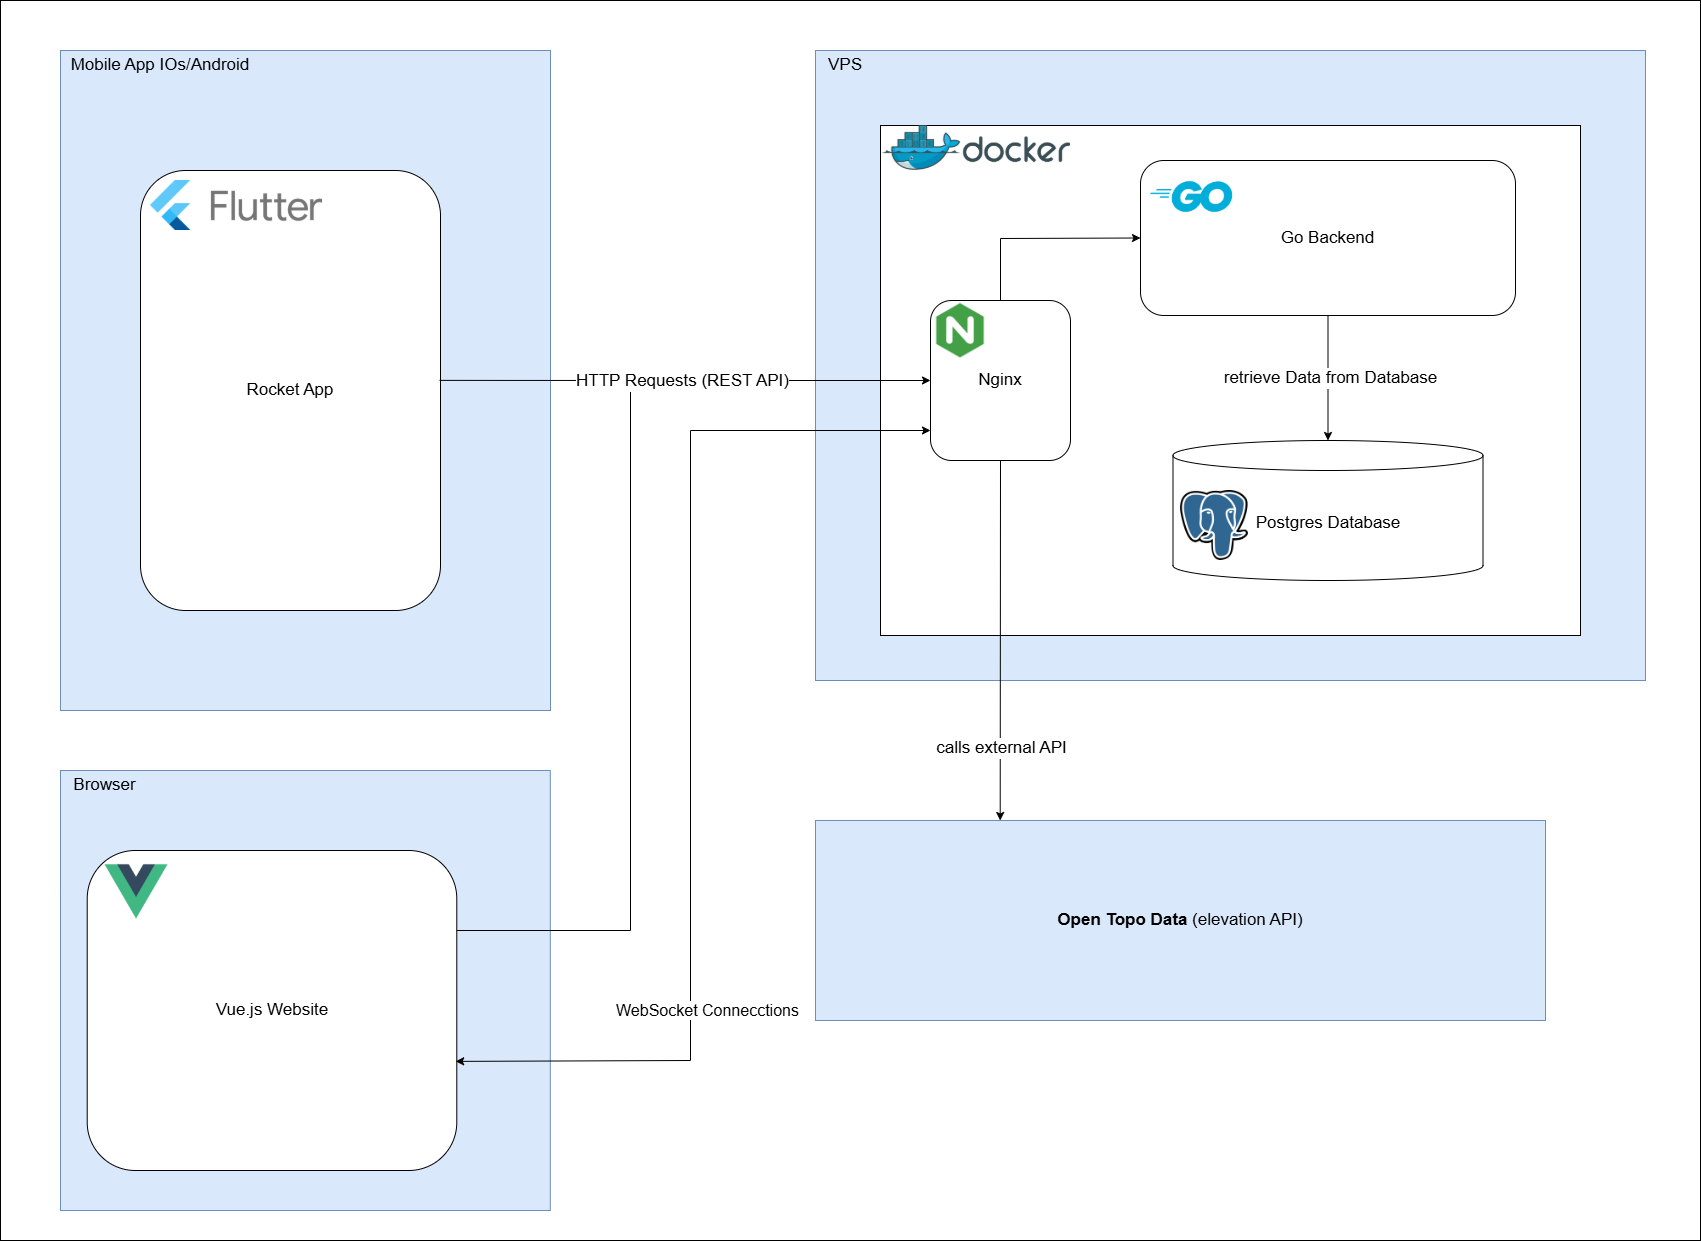
\includegraphics[width=0.95\textwidth]{images/HttpsArchitektur.png}
    \caption{Produktivarchitektur mit Docker, Nginx und HTTPS}
    \label{fig:https-architektur}
\end{figure}

\paragraph{Flutter Mobile App}
Die \textbf{Rocket App}, entwickelt mit dem Flutter Framework\cite{flutter}, läuft auf iOS und Android. Sie dient als Hauptschnittstelle für die Nutzer. Flutter wurde gewählt, weil es eine performante, plattformübergreifende Entwicklung mit einer Codebasis ermöglicht und gleichzeitig native App-Erlebnisse bietet.

Die App sendet ihre Daten  über REST-API-Aufrufe direkt an den VPS. Dabei handelt es sich um typische Aktionen wie das Hochladen von Läufen, Synchronisieren von Schritten, Highscorelisten oder das Abrufen von Challenges.

\paragraph{VPS und Containerisierung}
Der gesamte produktive Stack läuft auf einem \textbf{VPS (Virtual Private Server)}. Dies bietet volle Kontrolle über die Serverumgebung bei gleichzeitig moderaten Kosten.

Im VPS sind alle Backend-Komponenten mithilfe von \textbf{Docker}\cite{docker} containerisiert. Docker erlaubt es, die Applikation isoliert, portabel und versionssicher zu betreiben. Dies erleichtert auch das Deployment (z.\,B. durch GitHub Actions\cite{github}) sowie die Wartung im laufenden Betrieb.

\paragraph{Nginx als Reverse Proxy}
Als erste Instanz innerhalb des VPS fungiert \textbf{Nginx}\cite{nginx}. Dieser Reverse Proxy nimmt eingehende HTTP(S)-Anfragen entgegen, kümmert sich um SSL/TLS-Verschlüsselung (z.\,B. mit Let's Encrypt) und leitet die Anfragen an den Go-Backend-Container weiter.

Die Verwendung von Nginx bringt mehrere Vorteile:
\begin{itemize}
    \item Trennung von HTTPS-Terminierung und Backend-Logik
    \item Unterstützung von statischen Dateien und Caching
    \item Flexible Weiterleitung und Lastverteilung
\end{itemize}

\paragraph{Go Backend}
Das \textbf{Go-Backend} ist der Kern der Serverlogik. Es verarbeitet alle Anfragen der Mobile App über REST-Schnittstellen. Go\cite{golang} wurde gewählt wegen seiner hervorragenden Performance, statischen Typisierung, geringen Laufzeitanforderungen und der guten Eignung für API-Services.

Typische Funktionen des Go-Backends sind:
\begin{itemize}
    \item Verarbeiten und Speichern von Läufen, Schritten, Chats
    \item Authentifizierung und Benutzerverwaltung
    \item Bereitstellen von Geo- und Statistikdaten
\end{itemize}

\paragraph{PostgreSQL Datenbank}
Alle persistenten Daten werden in einer \textbf{PostgreSQL-Datenbank}\cite{postgresql} gespeichert. PostgreSQL wurde aufgrund seiner Zuverlässigkeit, SQL-Kompatibilität und Unterstützung von Geodaten (PostGIS) ausgewählt. Es läuft ebenfalls als Docker-Container innerhalb des VPS-Netzwerks.

\paragraph{Weitere Komponenten (kurz)}
Die \textbf{Vue.js-Webseite}\cite{vuejs}, ebenfalls im Bild dargestellt, kommuniziert wie die App mit dem Backend. Zusätzlich nutzt sie WebSockets für Live-Interaktionen. Eine externe Schnittstelle – hier die \textbf{OpenTopoData API}\cite{open_topo_data} – wird vom Backend genutzt, um Höhendaten für Strecken zu ermitteln.

\paragraph{Zusammenfassung der Architekturvorteile}
\begin{itemize}
    \item \textbf{Flutter:}\cite{flutter} Plattformübergreifende Entwicklung mit nativem Look \& Feel
    \item \textbf{Go:}\cite{golang} Hochperformant, ideal für APIs
    \item \textbf{Docker:}\cite{docker} Portabilität, einfache Updates und Isolierung
    \item \textbf{Nginx:}\cite{nginx} Reverse Proxy für Sicherheit und Routing
    \item \textbf{PostgreSQL:}\cite{postgresql} Robuste, erweiterbare SQL-Datenbank mit Geo-Support
\end{itemize}

\subsection{Lokale Entwicklungsarchitektur}
\label{sec:lokale-entwicklung}

\subsubsection{Unterschied zur Produktionsumgebung}

Die lokale Entwicklungsumgebung ist eine vereinfachte Version der Produktivarchitektur. Ziel ist es, einzelne Komponenten unabhängig testen und entwickeln zu können, ohne direkt ein Deployment auf dem VPS durchführen zu müssen.

Im Gegensatz zur vollständigen Produktionsarchitektur (siehe Abbildung \ref{fig:https-architektur}), bei der mehrere Docker-Container über einen Nginx-Reverse-Proxy orchestriert werden, wird in der lokalen Umgebung lediglich das Backend mit der zugehörigen Datenbank als \textbf{lokaler Docker-Container} betrieben.

\subsubsection{Architektur der lokalen Umgebung}
\begin{figure}[H]
    \centering
    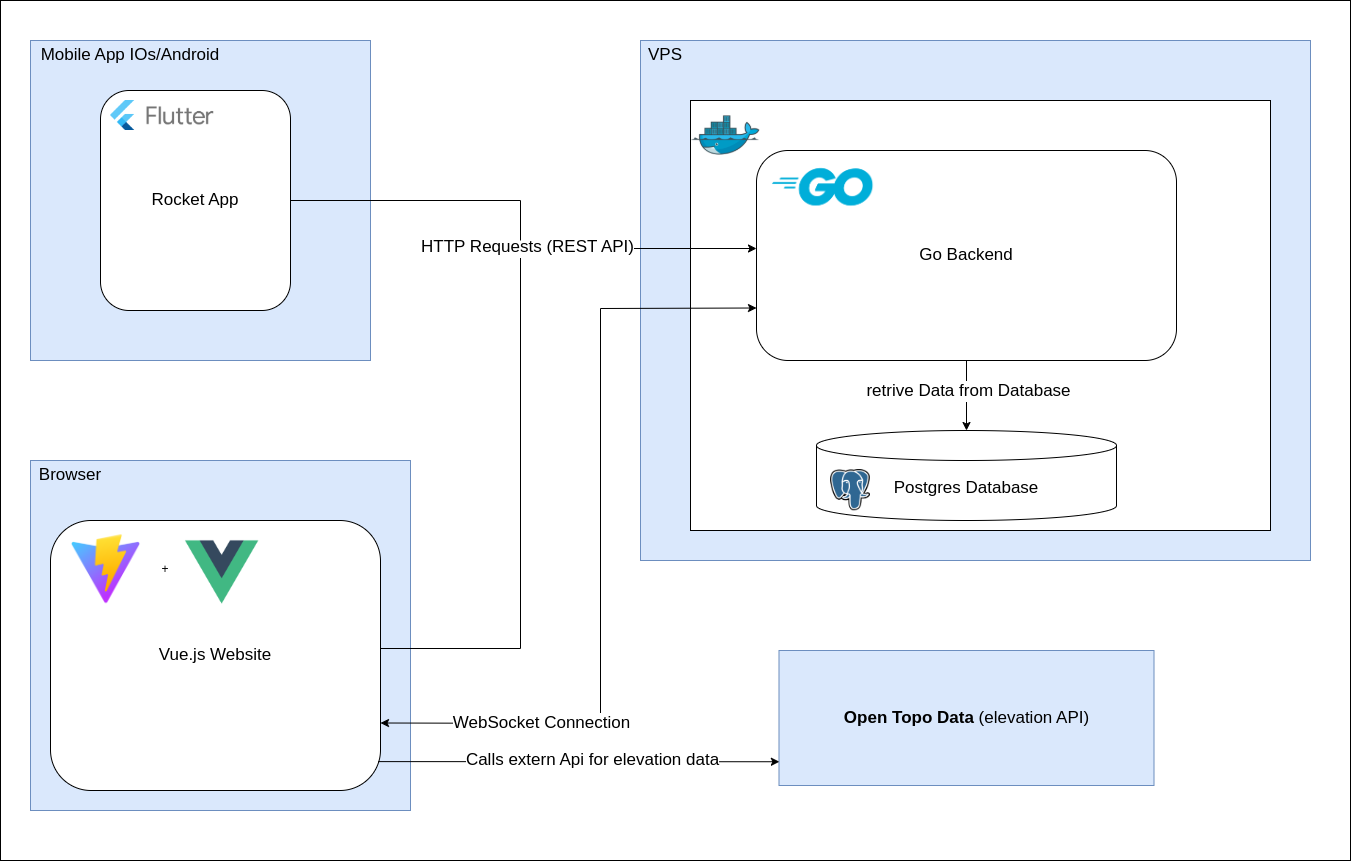
\includegraphics[width=0.9\textwidth]{images/Architecture.png}
    \caption{Lokale Entwicklungsumgebung}
    \label{fig:local-architektur}
\end{figure}

\paragraph{Backend \& Datenbank}
Das Go-Backend wird lokal in einem Docker-Container\cite{docker} gestartet, ebenso wie eine PostgreSQL-Datenbank\cite{postgresql} mit PostGIS-Erweiterung. Dadurch wird eine konsistente Entwicklungsumgebung geschaffen, die der produktiven Struktur sehr nahekommt, jedoch ohne HTTPS-Absicherung oder externe Abhängigkeiten wie Nginx\cite{nginx}.

\paragraph{Mobile App (Flutter)}
Die Mobile App kann über USB oder WLAN direkt auf einem realen Gerät installiert werden. Die Verwendung eines echten Geräts ist zwingend notwendig, da die App auf Geo-Koordinaten (GPS) und Schrittzählerdaten zugreift, welche über Gerätesensoren bereitgestellt werden. Emulatoren liefern keine oder nur ungenaue Sensorwerte und sind daher für Entwicklung und Tests ungeeignet. Für das Schrittzählen wird das Plugin \texttt{pedometer}\cite{pedometer} verwendet.

\paragraph{Web-Frontend (Vue.js + Vite)}
Das Web-Frontend basiert auf Vue.js\cite{vuejs} und kann ohne Docker lokal gestartet werden. Dazu wird der \textbf{Vite Development Server}\cite{vite} verwendet. Dieser bietet schnelles Hot Reloading und ist leichtgewichtig. Eine wichtige Besonderheit ist die Verwendung eines \textbf{Proxy-Setups}, das API-Anfragen aus dem Browser zur lokal laufenden Go-API weiterleitet. Dadurch können Frontend und Backend unabhängig voneinander entwickelt werden, ohne auf ein Deployment angewiesen zu sein.

\subsection{Backend Testing}

Für das Go-Backend existiert eine umfassende Teststrategie, die auf \textbf{Integrationstests} basiert. Ziel ist es, nicht nur die einzelnen Funktionen isoliert zu testen, sondern auch das Zusammenspiel zwischen REST-Endpunkten und Datenbankabfragen realistisch zu überprüfen.

\paragraph{Verwendete Tools}
Zum Schreiben und Ausführen der Tests kommen zwei populäre Go-Testbibliotheken zum Einsatz:
\begin{itemize}
    \item \texttt{github.com/onsi/ginkgo/v2}\cite{ginkgo} – Framework für Behavior-Driven Development (BDD)
    \item \texttt{github.com/onsi/gomega}\cite{gomega} – Assertion-Bibliothek für lesbare und präzise Testausdrücke
\end{itemize}

\paragraph{Isolierte Testumgebung mit Testcontainers}
Zur Laufzeit der Tests wird mit Hilfe von \texttt{testcontainers-go}\cite{testcontainers} eine isolierte Datenbankinstanz in einem temporären Docker-Container\cite{docker} gestartet. Diese Testdatenbank wird automatisch erstellt, mit den notwendigen Migrationsskripten versehen und nach jedem Testlauf vollständig bereinigt.

Dadurch ist sichergestellt, dass:
\begin{itemize}
    \item Jeder Test in einer identischen, kontrollierten Umgebung läuft
    \item Seiteneffekte zwischen Tests ausgeschlossen sind
    \item Produktivdaten niemals verwendet oder überschrieben werden
\end{itemize}

\paragraph{Testabdeckung}
Getestet werden:
\begin{itemize}
    \item Alle REST-Endpunkte des Backends
    \item Validierung und Fehlerfälle
    \item Alle relevanten Datenbankoperationen (CRUD)
\end{itemize}

Diese Teststrategie ermöglicht es, Änderungen im Backend schnell und sicher zu überprüfen, ohne dass manuelles Testen notwendig ist. Sie dient auch als wichtige Grundlage für zukünftige CI/CD-Pipelines.

\paragraph{Automatisierte Testausführung bei Pull Requests}
Alle Tests werden automatisch ausgeführt, sobald ein Pull Request (PR) auf den \texttt{master}-Branch erstellt wird. Dies erfolgt über eine GitHub Action, die das Test-Backend in einer isolierten Umgebung ausführt. Ein PR kann nur gemerged werden, wenn alle Tests erfolgreich durchlaufen. Dies garantiert, dass:
\begin{itemize}
    \item keine fehlerhaften Änderungen in die Hauptentwicklungslinie gelangen,
    \item alle Funktionen weiterhin wie erwartet funktionieren,
    \item die Softwarequalität über alle Sprints hinweg erhalten bleibt.
\end{itemize}


\section{ER-Modell und Datenbankarchitektur}

Die Anwendung verwendet \textbf{PostgreSQL}\cite{postgresql} als relationale Datenbank, ergänzt durch zwei wichtige Erweiterungen:

\begin{itemize}
    \item \textbf{PostGIS}: Ermöglicht die Speicherung und Verarbeitung von Geodaten, insbesondere Routeninformationen als \texttt{LINESTRING}. Diese werden für Laufstrecken und geplante Routen benötigt.
    \item \textbf{pgcrypto}: Wird zur Generierung von \texttt{UUIDs} (Universally Unique Identifiers) genutzt, die als Primärschlüssel in fast allen Tabellen verwendet werden.
\end{itemize}

Die Entscheidung für UUIDs anstelle klassischer Integer-IDs beruht auf mehreren Vorteilen:
\begin{itemize}
    \item \textbf{Sicherheit}: UUIDs sind schwer zu erraten und dadurch weniger anfällig für gezielte Angriffe über ID-Inkremente.
    \item \textbf{Skalierbarkeit}: Sie ermöglichen das Erstellen von IDs über verschiedene Systeme hinweg, ohne Kollisionen befürchten zu müssen.
    \item \textbf{Unabhängigkeit von Kontexten}: Da UUIDs global eindeutig sind, kann etwa eine Laufstrecke unabhängig vom Nutzer eindeutig referenziert werden.
\end{itemize}

\begin{figure}[H]
    \centering
    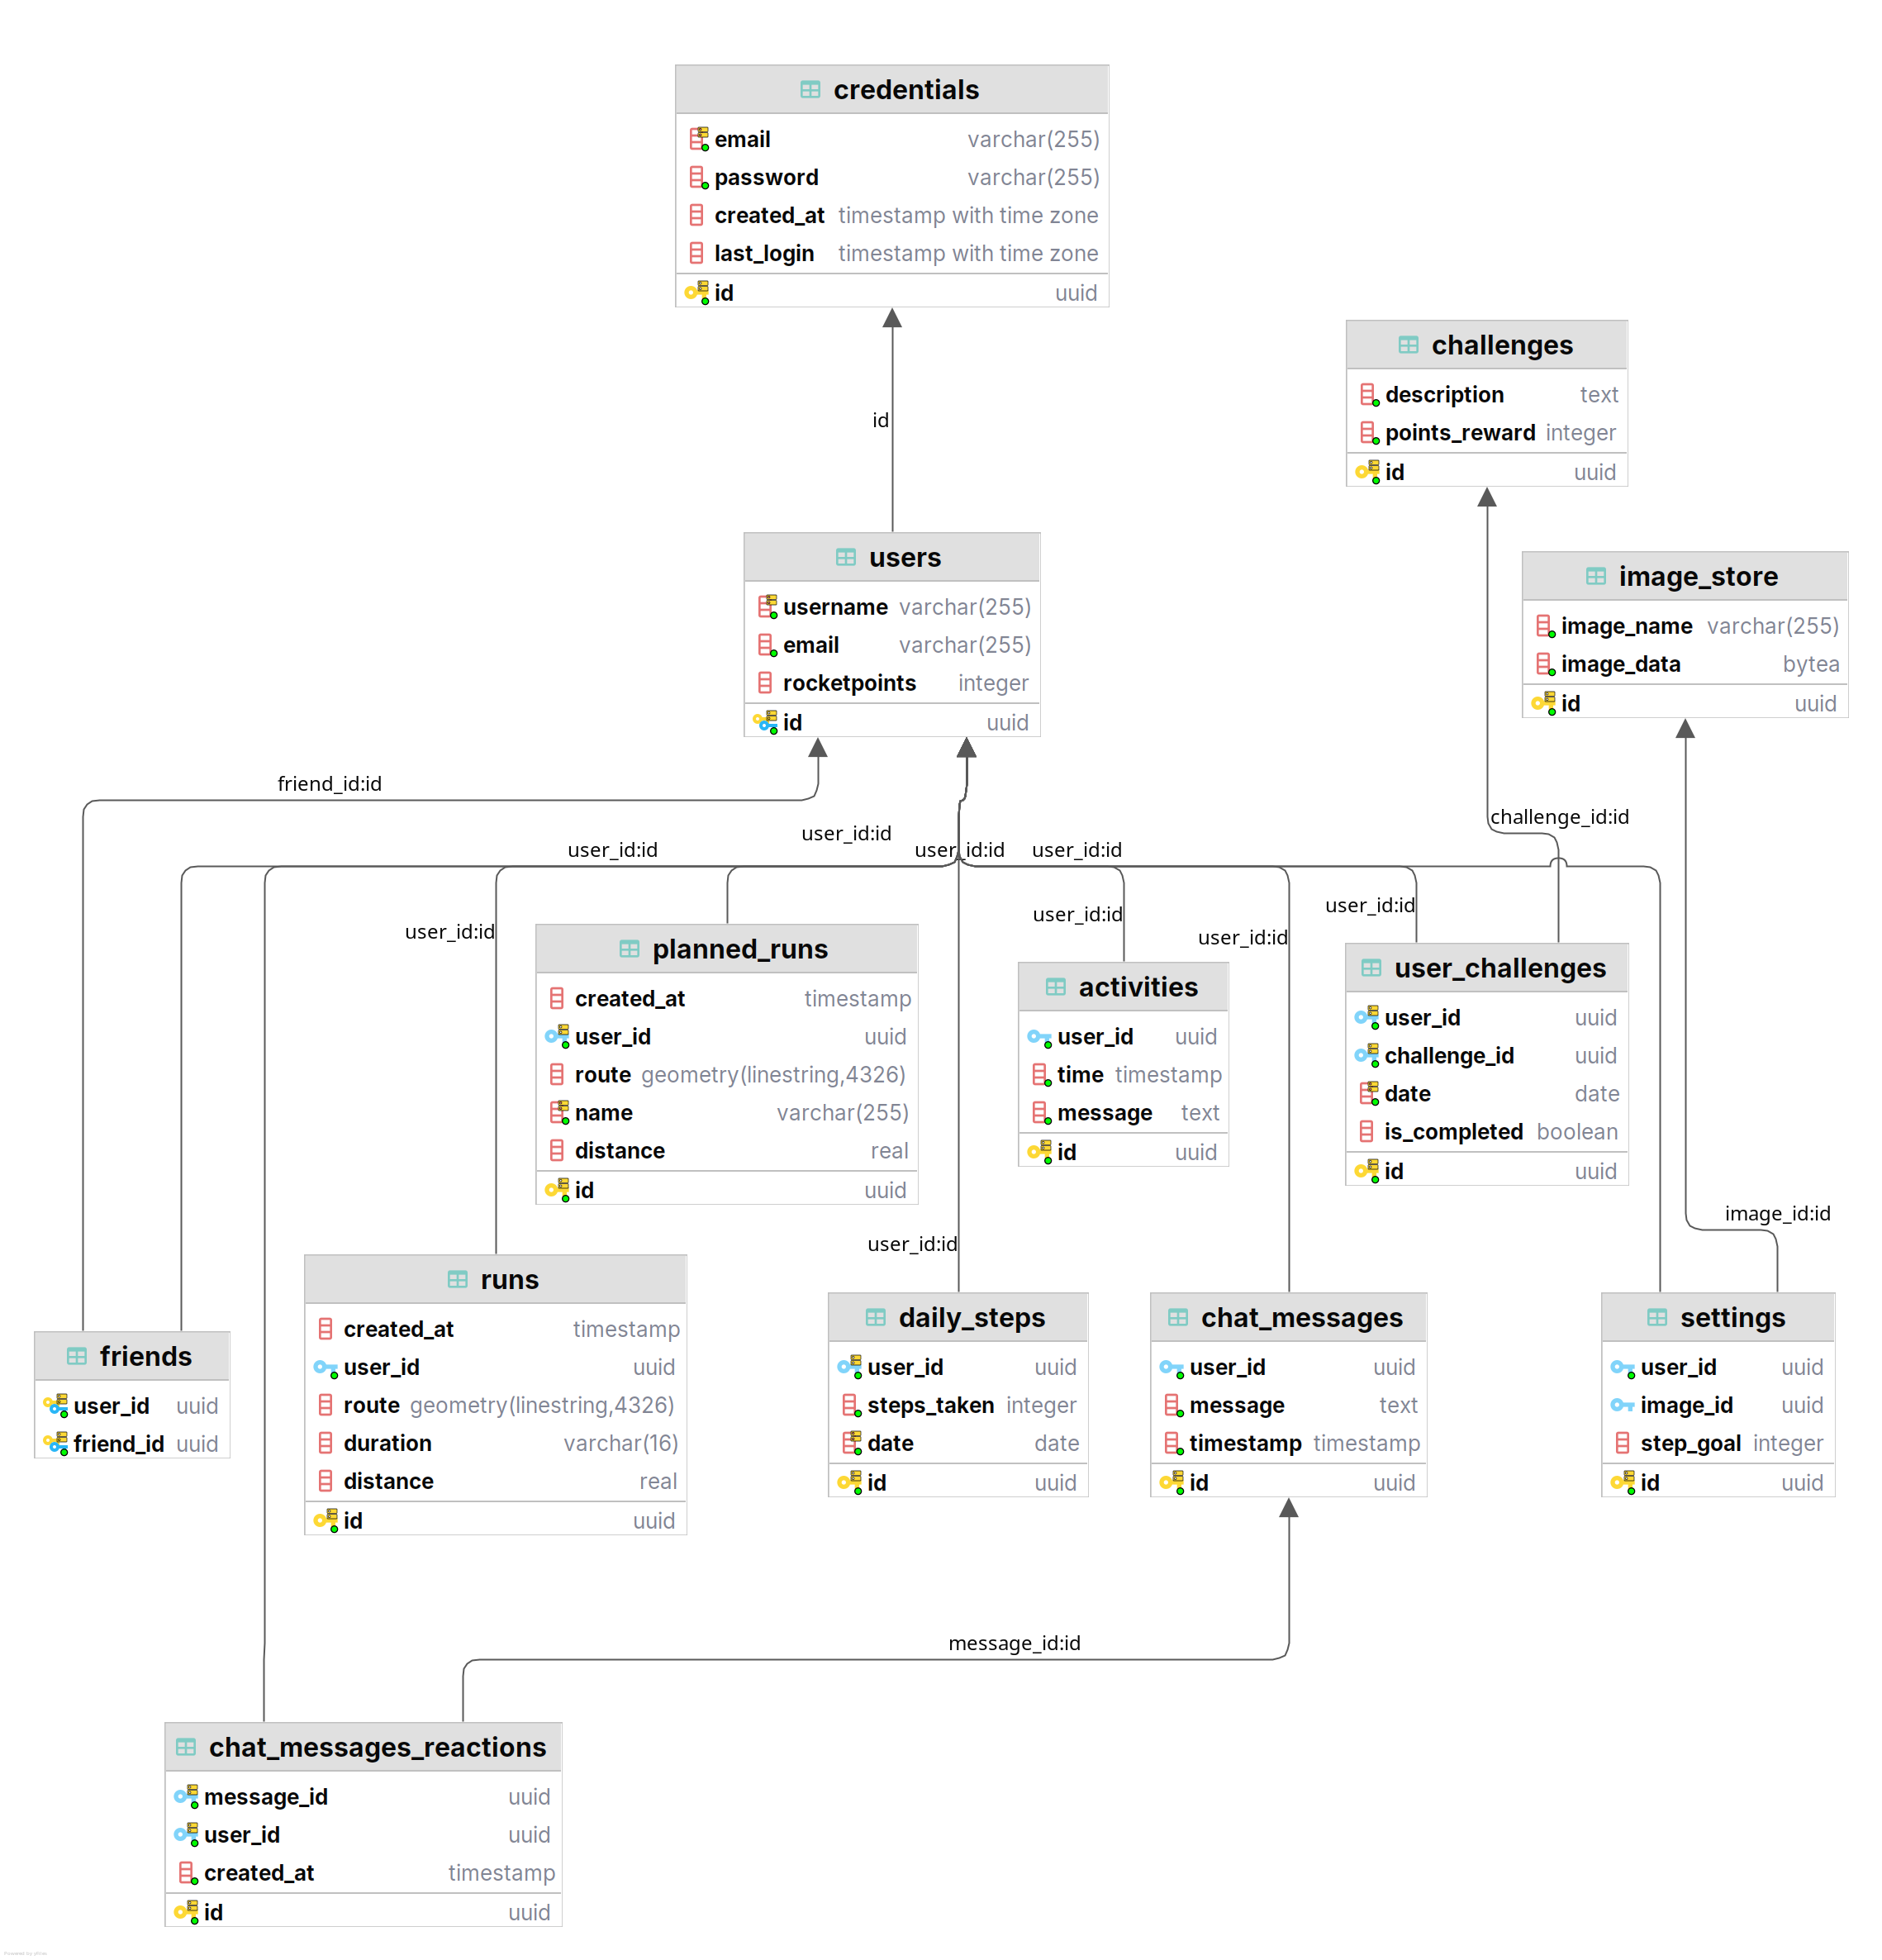
\includegraphics[width=0.8\linewidth]{images/RocketERLight.png}
    \caption{ER-Modell der Rocket-Anwendung}
\end{figure}

\begin{itemize}
    \item \textbf{users} – Zentrale Entität für Nutzer:innen der App. Enthält Username, Email und den Punktestand (Rocketpoints).
    \item \textbf{credentials} – Separat gespeicherte Zugangsdaten (E-Mail, Passwort) zur besseren Trennung von Authentifizierungs- und Nutzungsdaten.
    \item \textbf{planned\_runs} – Beinhaltet vom Nutzer vorgeplante Routen (mit Geometrie), Name und Ziel-Distanz. Essentiell für die Trainingsplanung.
    \item \textbf{runs} – Tatsächlich durchgeführte Läufe, ebenfalls mit Geodaten, Distanz und Dauer. Grundlage für Fortschrittsverfolgung.
    \item \textbf{daily\_steps} – Aggregierte tägliche Schrittzahlen pro Nutzer, oft durch Sensorschnittstellen (z.\,B. Mobilgerät) geliefert.
    \item \textbf{activities} – Logbuch-Funktion für allgemeine Nutzeraktionen. Enthält Textnachrichten und Zeitstempel.
    \item \textbf{friends} – Bidirektionale Freundschaften zwischen Nutzer:innen. Erlaubt soziales Tracking und Interaktion.
    \item \textbf{challenges} – Vorgedefinierte Herausforderungen mit Beschreibung und Punktebelohnung.
    \item \textbf{user\_challenges} – Relationstabelle zwischen Nutzer:innen und Herausforderungen, inkl. Statusinformationen wie \texttt{is\_completed}.
    \item \textbf{settings} – Benutzerbezogene Konfigurationen, insbesondere Zielwerte wie Schrittanzahl oder Profilbild.
    \item \textbf{image\_store} – Speicherung binärer Bilddaten (z.\,B. Avatare, Challenge-Bilder). Gekoppelt an andere Tabellen über \texttt{image\_id}.
    \item \textbf{chat\_messages} – Ermöglicht einfache Nachrichten zwischen Nutzer:innen. Repräsentiert den sozialen Aspekt der App.
    \item \textbf{chat\_messages\_reactions} – Erweiterung für Reaktionen (z.\,B. Emojis) auf Chatnachrichten. Enthält Zeitstempel und Verweis auf Nutzer:in.
\end{itemize}

Alle Relationen sind über \texttt{uuid}-Fremdschlüssel miteinander verknüpft, was eine klare logische Trennung und Erweiterbarkeit des Systems unterstützt. Die Kombination aus Geodaten, sozialen Funktionen und gamifizierter Nutzerinteraktion bildet das Rückgrat der Applikation.


\section{Authentifizierung und User Validierung}

Für die Authentifizierung und Validierung der Nutzer setzen wir auf JSON Web Tokens (JWT). JWT ermöglicht eine sichere und effiziente Methode, um Benutzeridentitäten zwischen Client und Server zu verifizieren, ohne bei jeder Anfrage die Datenbank abfragen zu müssen.

Der große Vorteil von JWT liegt darin, dass alle nötigen Informationen in einem signierten Token gebündelt sind, das sowohl Integrität als auch Authentizität gewährleistet. Dies reduziert die Serverlast und ermöglicht gleichzeitig eine skalierbare und stateless-Authentifizierung.

In unserer Architektur unterscheiden wir die Handhabung des Tokens zwischen App und Web:

\begin{itemize}
    \item \textbf{Mobile App:} Hier wird der JWT-Token nach erfolgreichem Login sicher im \texttt{SecureStorage} gespeichert, um ihn bei nachfolgenden API-Anfragen im Header mitzuschicken. Das Plugin \texttt{flutter\_secure\_storage}\cite{flutter_secure_storage} gewährleistet, dass der Token verschlüsselt und vor unbefugtem Zugriff geschützt ist. Ein Beispiel zur Speicherung sieht folgendermaßen aus:

\begin{lstlisting}[language=Dart, caption=Speichern des JWT Tokens im Secure Storage]
await _storage.write(key: 'jwt_token', value: loginResponse.token);
\end{lstlisting}

    \item \textbf{Webanwendung:} Im Browser wird der JWT-Token als HTTP-Cookie verwaltet. Dies ermöglicht eine einfache automatische Übertragung bei Anfragen und reduziert die Notwendigkeit, den Token manuell im Header zu setzen.
\end{itemize}

Alle API-Endpunkte außer \texttt{/login} und \texttt{/register} sind als \textit{protected routes} konfiguriert. Das bedeutet, dass jede Anfrage an diese Endpunkte nur mit einem gültigen JWT im Header akzeptiert wird. Auf diese Weise verhindern wir, dass unautorisierte Nutzer auf geschützte Daten zugreifen können.

Beim Fehlen eines gültigen Tokens oder bei einem abgelaufenen Token wird der Zugriff verweigert und ein entsprechender Fehler (z.B. HTTP 401 Unauthorized) zurückgegeben. Dieses Vorgehen stellt sicher, dass sensible Daten und Funktionen nur authentifizierten Benutzern zugänglich sind.

Der Authentifizierungs-Workflow ist in Abbildung~\ref{fig:validation-workflow} schematisch dargestellt.

\begin{figure}[H]
    \centering
    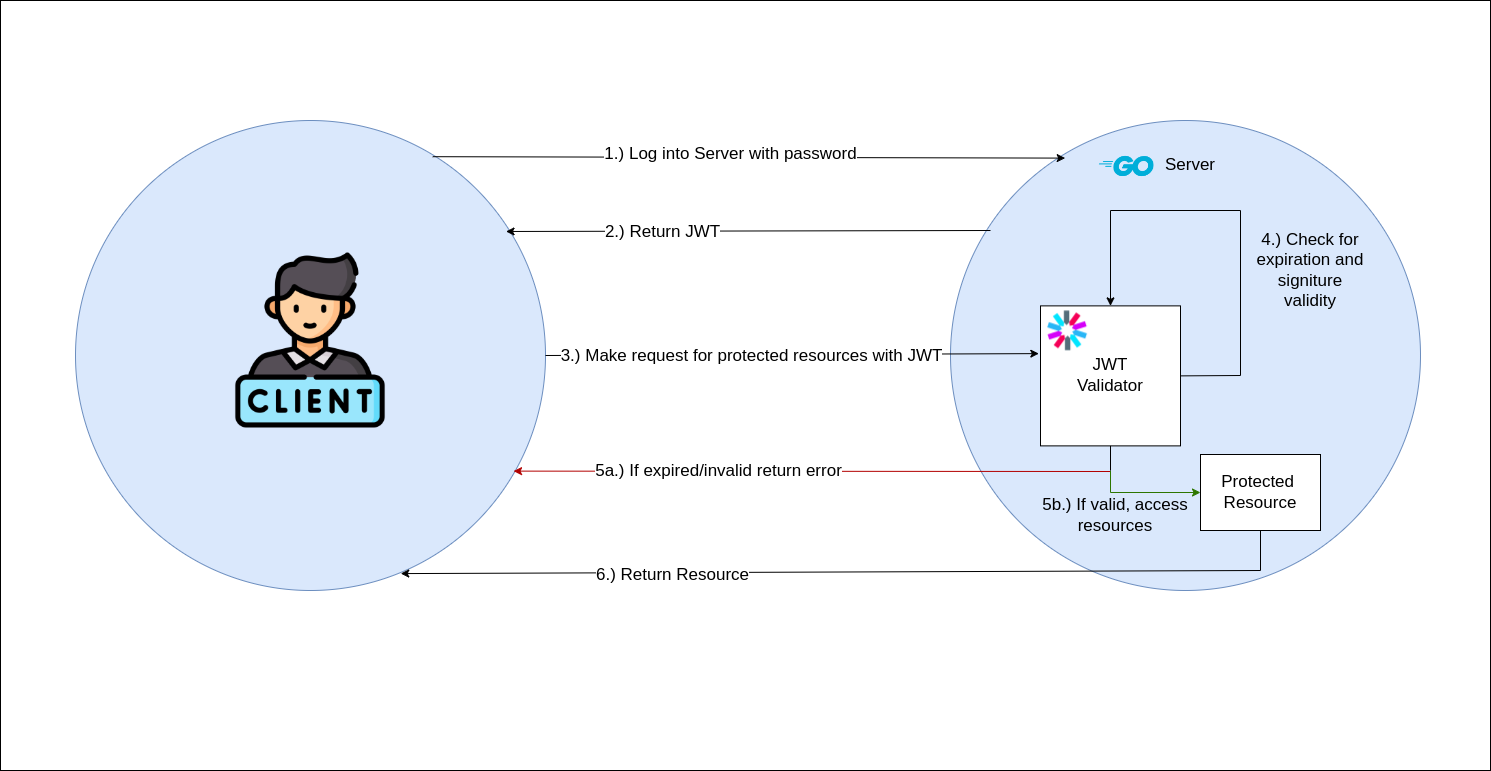
\includegraphics[width=0.9\textwidth]{images/ValidationWorkflow.png}
    \caption{Workflow der Nutzer-Validierung mittels JWT}
    \label{fig:validation-workflow}
\end{figure}

Die Entscheidung für JWT fiel aufgrund der folgenden Gründe:
\begin{itemize}
    \item \textbf{Skalierbarkeit:} Da JWT stateless ist, muss der Server keine Sitzungsdaten speichern, was die Skalierung der Anwendung erleichtert.
    \item \textbf{Sicherheit:} Durch die Signatur des Tokens wird sichergestellt, dass der Token nicht manipuliert wurde.
    \item \textbf{Flexibilität:} JWT kann problemlos in verschiedenen Client-Typen (Mobile, Web) genutzt werden und erlaubt verschiedene Nutzlasten (Claims).
\end{itemize}

Durch diese Implementierung gewährleisten wir eine sichere, performante und flexible Authentifizierung, die sich nahtlos in unsere Cross-Plattform-Lösung integriert.




\section{Handy App}
\subsection{Foreground Task}

Die App verwendet das Flutter-Plugin \texttt{flutter\_foreground\_task}\cite{flutter_foreground_task}, um dauerhaft im Vordergrund bzw. Hintergrund Schrittzahlen zu erfassen und regelmäßig an das Backend zu senden. Dies ist vor allem unter Android notwendig, da das Betriebssystem Hintergrundprozesse stark einschränkt und andernfalls wichtige Trackingdaten verloren gehen könnten.

Die Foreground Task besteht aus zwei getrennten Instanzen, welche in unterschiedlichen Isolates (Flutter-Threads) laufen. Diese kommunizieren nicht direkt über Speicher, sondern über Ports:

\begin{itemize}[leftmargin=1.5em]
    \item \textbf{Hauptanwendung (Main Isolate)}: Dies ist der Hauptthread, in dem auch die Benutzeroberfläche läuft. Dort wird der Foreground-Task initialisiert und gestartet.
\end{itemize}

\begin{lstlisting}[language=Dart, caption=Initialisierung des Foreground Task]
FlutterForegroundTask.initCommunicationPort();
_initService();
await _startService();
\end{lstlisting}

\begin{lstlisting}[language=Dart, caption=Registrierung des Task Handlers]
@pragma('vm:entry-point')
void startCallback() {
  FlutterForegroundTask.setTaskHandler(MyTaskHandler());
}
\end{lstlisting}

\begin{itemize}[leftmargin=1.5em]
    \item \textbf{Hintergrundprozess (TaskHandler Isolate)}: Die Klasse \texttt{MyTaskHandler} implementiert den Hintergrunddienst. Dieser läuft in einem separaten Isolate, das keine direkte Verbindung zur Hauptanwendung hat. Die wichtigsten Aufgaben des TaskHandlers sind:
    \begin{itemize}
        \item Schrittzählung mit dem Plugin \texttt{pedometer}\cite{pedometer}
        \item Tageswechsel erkennen und Schritte zurücksetzen
        \item Regelmäßige Synchronisierung mit dem Backend alle 15 Minuten
    \end{itemize}
\end{itemize}

\begin{lstlisting}[language=Dart, caption=Schrittzählung starten]
_sub = Pedometer.stepCountStream.listen(_onStepCount);
\end{lstlisting}

\begin{lstlisting}[language=Dart, caption=Tageswechsel erkennen]
if (!_isSameDay(now, _lastResetDate)) {
  _baselineSteps = event.steps;
  _stepsToday = 0;
}
\end{lstlisting}

\begin{lstlisting}[language=Dart, caption=Synchronisierung mit dem Backend]
await api.DailyStepsApi.sendDailySteps(steps, jwt);
\end{lstlisting}

\paragraph{Kommunikation zwischen Instanzen}
Da Haupt- und Hintergrundprozess getrennt sind, wird der JWT-Token über eine Nachricht übertragen und im SharedPreferences-Store abgelegt. Ebenso werden Schrittzahlen regelmäßig an die Hauptinstanz gemeldet. Dies geschieht über:

\begin{lstlisting}[language=Dart, caption=Schritte an Hauptprozess senden]
FlutterForegroundTask.sendDataToMain(_stepsToday);
\end{lstlisting}

Es ist wichtig zu verstehen, dass diese Trennung notwendig ist, aber auch eine gewisse Komplexität mit sich bringt – z.B. bei der Persistierung von Zuständen oder dem Teilen von Authentifizierungsinformationen.

\paragraph{Berechtigungen}
Damit der Foreground Task korrekt ausgeführt werden kann, sind verschiedene Berechtigungen notwendig:

\begin{itemize}
    \item Notification-Permission
    \item Aktivitätserkennung (für Schrittzählung)
    \item Optional: Deaktivieren von Battery-Optimierung (vorbereitet, aber auskommentiert)
\end{itemize}

\begin{lstlisting}[language=Dart, caption=Abfrage der Berechtigungen]
if (Platform.isAndroid) {
  if (await Permission.activityRecognition.isDenied) {
    await Permission.activityRecognition.request();
  }
}
\end{lstlisting}

Dieser Foreground Task bildet die Grundlage für die dauerhafte Aktivitätsaufzeichnung und ermöglicht eine robuste Synchronisation mit dem Backend – unabhängig davon, ob sich die App im Vorder- oder Hintergrund befindet.


\subsection{Tracking und Anzeige von Lauf-Routen}

In unserer App wird die Lauf-Route eines Nutzers kontinuierlich mithilfe von GPS-Daten erfasst. Diese Positionsdaten werden als \textit{GeoPoints} gespeichert, um später die gesamte Laufstrecke rekonstruieren und visualisieren zu können.

\subsubsection{Verwendung von OpenStreetMap}

Für die Darstellung der Routen auf der Karte setzen wir die Open-Source-Kartenplattform \textit{OpenStreetMap} (OSM)\cite{openstreetmap} ein. Die Flutter-Bibliothek \texttt{flutter\_osm\_plugin}\cite{flutter_osm_plugin} ermöglicht die nahtlose Integration der OSM-Karten in die App und bietet umfangreiche Funktionen, wie z.B. das Zeichnen von Wegen, die Anzeige von Markern und Nutzerpositionen.

OSM bietet den Vorteil, dass die Kartendaten frei verfügbar und anpassbar sind. So können wir die Laufstrecke direkt auf der Karte abbilden, indem wir die gesammelten Geo-Koordinaten als Pfad über die Karte legen.

\subsubsection{Erfassung und Speicherung der GPS-Daten}

Während eines Laufs werden fortlaufend die aktuellen GPS-Koordinaten des Nutzers abgefragt. Diese Koordinaten werden in einer Liste von \texttt{GeoPoint} Objekten gesammelt, die jeweils die \texttt{latitude} und \texttt{longitude} enthalten.

\begin{lstlisting}[language=Dart, caption=Hinzufügen eines GeoPoints zur Route]
_routePoints.add(GeoPoint(
  latitude: position.latitude,
  longitude: position.longitude,
));
\end{lstlisting}

Diese Liste bildet die gesamte Laufstrecke ab. Neben den Geo-Koordinaten wird die verstrichene Zeit mit einem Timer gemessen und später zusammen mit der Route gespeichert.

\subsubsection{Senden der Route an das Backend}

Um die Laufdaten dauerhaft zu speichern, werden die Geo-Punkte in ein standardisiertes Format, den sogenannten \texttt{LINESTRING}, umgewandelt. Dieses Format wird häufig in geografischen Informationssystemen (GIS) verwendet, um Linien oder Wege zu repräsentieren.

\begin{lstlisting}[language=Dart, caption=Erzeugen eines LINESTRINGs]
String lineString = 'LINESTRING(' +
  _routePoints.map((p) => '${p.longitude} ${p.latitude}').join(', ') +
  ')';
\end{lstlisting}

Die Umwandlung ist notwendig, damit das Backend die Route als eine durchgehende Linie interpretieren kann. Anschließend wird der \texttt{LINESTRING} zusammen mit der Laufzeit an die API gesendet:

\begin{lstlisting}[language=Dart, caption=Senden der Laufdaten ans Backend]
await RunAPI.saveRun(lineString, _elapsedTime);
\end{lstlisting}

\subsubsection{Darstellung der Route in der App}

Zur Visualisierung der gespeicherten Laufstrecken wird die Route vom Backend geladen und als Liste von GeoPoints in der App dargestellt. Über die OpenStreetMap-Karte wird dann die Strecke mit der Funktion \texttt{drawRoad} gezeichnet.

Dabei werden die einzelnen Segmente der Route als Fußwege (RoadType.foot) mit einer roten Linie hervorgehoben:

\begin{lstlisting}[language=Dart, caption=Zeichnen der Route auf der Karte]
for (int i = 0; i < _routePoints.length - 1; i++) {
  await _mapController.drawRoad(
    _routePoints[i],
    _routePoints[i + 1],
    roadType: RoadType.foot,
    roadOption: RoadOption(
      roadColor: Colors.red,
      roadWidth: 8,
    ),
  );
}
\end{lstlisting}

Diese Visualisierung ermöglicht dem Nutzer, die genaue Strecke seines Laufs nachvollziehen zu können. Zusätzlich werden wichtige Informationen wie Gesamtdistanz und Laufzeit übersichtlich angezeigt.

\subsubsection{Berechnung der Gesamtdistanz}

Die Gesamtdistanz wird aus den GeoPoints berechnet, indem für jedes aufeinanderfolgende Punktpaar die Entfernung mithilfe der Haversine-Formel bestimmt wird. Diese Formel berechnet die kürzeste Entfernung über die Erdoberfläche zwischen zwei Koordinaten.

\begin{lstlisting}[language=Dart, caption=Berechnung der Entfernung zweier GeoPoints]
double _calculateDistanceBetween(GeoPoint a, GeoPoint b) {
  const double R = 6371; // Erdradius in Kilometern
  double dLat = _deg2rad(b.latitude - a.latitude);
  double dLon = _deg2rad(b.longitude - a.longitude);
  double lat1 = _deg2rad(a.latitude);
  double lat2 = _deg2rad(b.latitude);

  double hav = sin(dLat / 2) * sin(dLat / 2) +
      sin(dLon / 2) * sin(dLon / 2) * cos(lat1) * cos(lat2);
  double c = 2 * atan2(sqrt(hav), sqrt(1 - hav));
  return R * c;
}
\end{lstlisting}

Die Summe aller Teilstrecken ergibt die Gesamtstrecke des Laufs.

\newpage
\section{Referenzen}

\begin{thebibliography}{9}
\bibitem{androidstudio}
Android Studio, \emph{Android Studio IDE}, \url{https://developer.android.com/studio}

\bibitem{docker}
Docker, \emph{Docker: Empowering App Development for Developers}, \url{https://www.docker.com/}

\bibitem{flutter}
Flutter, \emph{Flutter - Beautiful native apps in record time}, \url{https://flutter.dev/}

\bibitem{flutter_foreground_task}
Flutter Foreground Task, \emph{Flutter Foreground Task Plugin}, \url{https://pub.dev/packages/flutter_foreground_task}

\bibitem{flutter_osm_plugin}
Flutter OSM Plugin, \emph{Flutter OSM Plugin for OpenStreetMap}, \url{https://pub.dev/packages/flutter_osm_plugin}

\bibitem{flutter_secure_storage}
Flutter Secure Storage, \emph{Flutter Secure Storage Plugin}, \url{https://pub.dev/packages/flutter_secure_storage}

\bibitem{ginkgo}
Ginkgo, \emph{Ginkgo: BDD Testing Framework for Go}, \url{https://onsi.github.io/ginkgo/}

\bibitem{github}
GitHub, \emph{GitHub: Where the world builds software}, \url{https://github.com/}

\bibitem{gomega}
Gomega, \emph{Gomega: Matcher Library for Go}, \url{https://onsi.github.io/gomega/}

\bibitem{golang}
Go, \emph{The Go Programming Language}, \url{https://golang.org/}

\bibitem{gopls}
Go Language Server Protocol, \emph{gopls: The Go Language Server}, \url{https://github.com/golang/tools/tree/master/gopls}

\bibitem{migrate}
Migrate, \emph{Migrate: Database Migration Tool}, \url{https://github.com/golang-migrate/migrate}

\bibitem{nginx}
NGINX, \emph{NGINX Web Server}, \url{https://nginx.org/}

\bibitem{open_topo_data}
OpenTopoData, \emph{OpenTopoData: Open Topographic Data}, \url{https://opentopodata.org/}

\bibitem{openstreetmap}
OpenStreetMap, \emph{OpenStreetMap Project}, \url{https://www.openstreetmap.org/}

\bibitem{pedometer}
Pedometer, \emph{Flutter Pedometer Plugin}, \url{https://pub.dev/packages/pedometer}

\bibitem{postgresql}
PostgreSQL, \emph{The World's Most Advanced Open Source Relational Database}, \url{https://www.postgresql.org/}

\bibitem{testcontainers}
Testcontainers, \emph{Testcontainers for Go}, \url{https://golang.testcontainers.org/}

\bibitem{vite}
Vite, \emph{Vite: Next Generation Frontend Tooling}, \url{https://vitejs.dev/}

\bibitem{vuejs}
Vue.js, \emph{Vue.js: The Progressive JavaScript Framework}, \url{https://vuejs.org/}

\bibitem{VSCode}
Visual Studio Code, \emph{Visual Studio Code: Code Editing. Redefined}, \url{https://code.visualstudio.com/}

\bibitem{zed}
Zed, \emph{Zed: A modern code editor}, \url{https://zed.dev/}

\end{thebibliography}

\end{document}
